\chapter{Background}
\lhead{\emph{Background}}

\section{Introduction to the History of Computer Vision}
\label{sec:intro}


Computer vision is a relatively old field in computer science. The subject itself has been around since the 1960s, but it is only recently that it has been possible to build useful computer systems ideas from computer vision \cite {cv}.
The birthday of Computer Vision is considered the summer of 1966.  During that year a computer vision summer project was proposed in MIT AI lab \citep{papert}. The goal of the summer vision project was to use summer workers (students) effectively in the construction of a significant part of a visual system. It was thought that a vision was a relatively easy field of AI and that a landmark in the development of pattern recognition could be created during the summer. The task, however, was a lot harder than previously expected and no significant computer vision problems were solved during that project.

During development of a computer vision, it was noticed that is very hard to recognize an object by describing the whole image because of the pixel variation in images that are produced under different conditions. Important features have to be selected to make an image more resistible to various variations. Later these selected features are used for detecting a specific object. In 1999 a new method for image feature generation called the Scale Invariant Feature Transform (SIFT) was proposed by \cite{sift}. These features are invariant to image scaling, translation, and rotation, and partially invariant to illumination changes. Because of that SIFT features performed much better than correlation-based template matching technique that was used before and could be seen as a major break point in computer vision.
 
Another method for detecting features in images was proposed by \citep{nakano2006object}. This paper states that since objects are composed of a combination of characteristic parts, a good object detector could be developed if local parts specialised for a detection target are derived automatically from training samples. To do this, Independent component analysis (ICA) was used which decomposes a signal into independent elementary signals. Then ICA vectors were applied to the candidate area and their outputs were used in classification. Using this approach face detector algorithm used in Fujifilm camera with real-time face detection was created. It is considered to be a first commercial application that could run computer vision algorithms in real time. 
 
The important turning point in the development of computer vision field was a creation of ImageNet dataset and the ImageNet Large Scale Visual Recognition Challenge in 2010. The challenge is a competition where research teams submit image classification algorithms that classify and detect objects and scenes. The challenge is running annually since 2010 \citep{ImageNet}. In 2010 the goal of the challenge was to estimate the content of photographs for the purpose of retrieval and automatic annotation using a subset of the large hand-labeled ImageNet dataset (10.000.000 labeled images depicting 10.000+ object categories) as the training set. Example images which represent a pizza class can be seen in \autoref{fig:imgnet}.


Because of a  big amount of images and categories ImageNet was and still is a huge challenge for researchers who compete in the challenge.  ImageNet encouraged improvement and innovation in computer vision techniques. In 2012 ImageNet competition was won by an approach that used convolutional neural networks- AlexNet \citep{alex}. Since then deep learning became a dominant method for an image classification. 


 \begin{figure}[h]
\centering
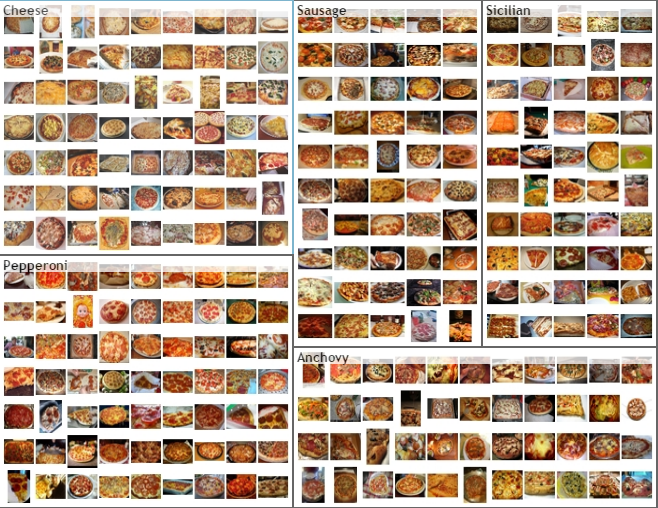
\includegraphics[width=10cm]{Figures/2/imgnet.PNG}
\caption{Example images with a pizza class label from the ImageNet }
\label{fig:imgnet}
\end{figure}


\section{Why is Computer Vision a Hard Problem?}
The true challenge to artificial intelligence proved to be solving the tasks that are easy for people to perform but hard for people to describe formally – problems that we solve intuitively, that feel automatic, like recognizing objects in images \citep{Goodfellow-et-al-2017}.

A human can recognize objects in images under all kinds of variations of illumination, viewpoint, scale, etc. In comparison, computer algorithms are very susceptible to all kinds of variations in images. Major variations in images were defined by \cite{231n} as:

\begin{enumerate}
\item Viewpoint variation. A single instance of an object can be oriented in many ways with respect to the camera.
\item Scale variation. Visual classes often exhibit variation in their size (size in the real world, not only in terms of their extent in the image).
\item Deformation. Many objects of interest are not rigid bodies and can be deformed in extreme ways.
\item Occlusion. The objects of interest can be occluded. Sometimes only a small portion of an object can be visible.
\item Illumination conditions. The effects of illumination are drastic on the pixel level.
\item Background clutter. The objects of interest may blend into their environment, making them hard to identify.
\item Intra-class variation. The classes of interest can often be relatively broad, such as a chair. There are many different types of these objects, each with their own appearance.
\end{enumerate}


 \begin{figure}[h]
\centering
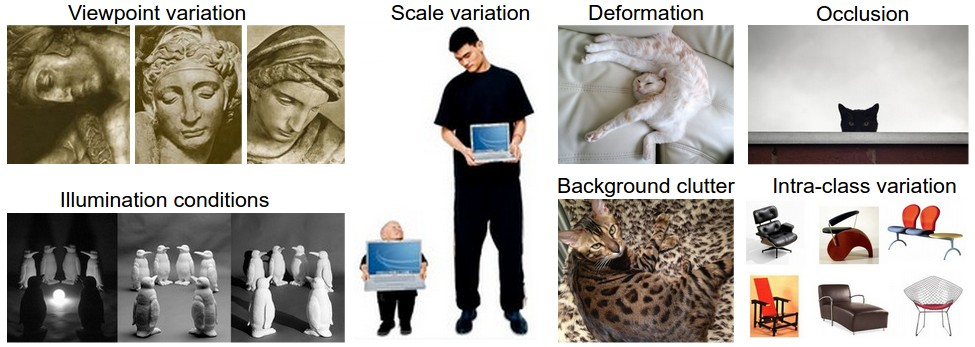
\includegraphics[width=14cm]{Figures/2/challenges.jpeg}
\caption{Example of various variations in images \citep{231n}}
\label{fig:imgnet}
\end{figure}

The actual solution of the variation problem still has not been found. Currently, this problem is either ignored or some algorithms that are partly resistant to variations are used.

\section{Saliency-aware Food Image Segmentation for Personal Dietary Assessment Using a Wearable Computer}
A computer system that can be used for an image-based dietary assessment was described by \cite{chen2015saliency}. A wearable computer called eButton is used to capture the eating events. The eButton is a small, unobtrusive chest fob that can be pinned to clothing on the chest. Its camera takes pictures automatically at a rate of one picture per second during eating events. Then segmentation techniques are applied to segment a food from a container. Finally, a person manually enters the food label to the application. Later food volume is estimated. There is no information about food volume measurement, nutrient database lookup and calculation of calories in the paper despite that these steps are shown in the eButton operational diagram. \autoref{fig:1}
\begin{figure}[ht]
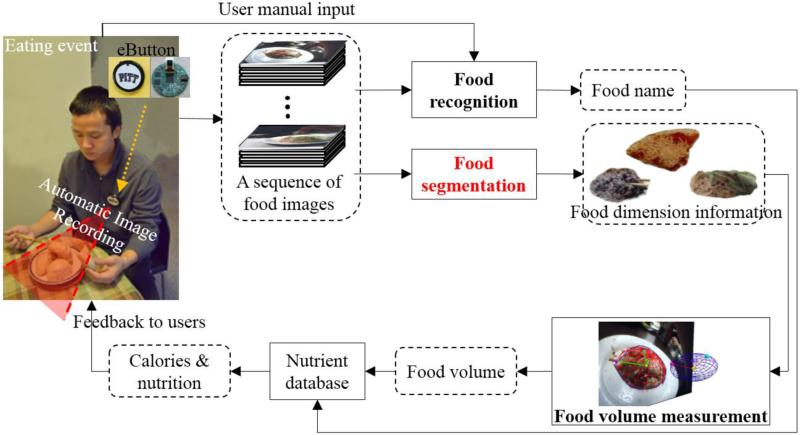
\includegraphics{Figures/segm_01.jpg}
\caption{Personal dietary assessment using a wearable computer eButton. }
\label{fig:1}
\end{figure}

The main focus of the paper is food segmentation from its container. It states that major difficulties in automatic food segmentation are multiple food components in complex and varying configurations, colored decorative patterns on plates and occlusion by non-food objects. The example images of these three difficulties are shown in  \autoref{fig:2}.

\begin{figure}[ht]
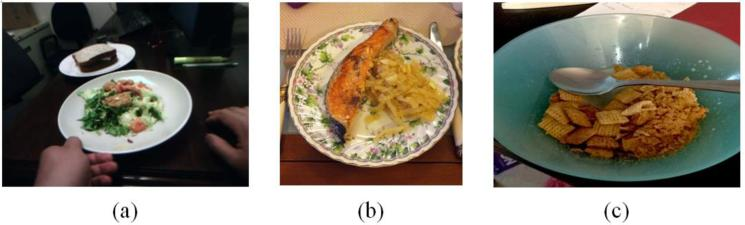
\includegraphics{Figures/segm_02.jpg}
\caption{Major difficulties in automatic food segmentation }
\label{fig:2}
\end{figure}

Researchers use two stages approach for food segmentation. Firstly, food container is detected in an image. The container is detected by shape convexity.  Canny edge detector is used to obtain the edge information from a given image.
Then, a number of square windows centered at edge pixels are randomly selected \label{fig:2}. A trained support vector machine with the histogram of a gradient as the classifier input is used to discard the non-container edge windows, increasing the detection efficiency. 

For detecting the food inside a plate researchers used color contrast to characterize the difference between the objects in the region against their surroundings, color abundance to characterise a probability of a color appearing in the local window and spatial arrangement to recognize the areas with one highly dominant color in the image. These 3 characteristics are then combined into one function.

The data set used to evaluate the segmentation approach in this research was combined from 30 eating events captured with eButton and 30 food images from the Jawbone database. Accuracy was measured by visually inspecting the quality of the segmentation and by comparing the image segmented by a computer to the images segmented by two research participants and measuring the difference. 



\begin{figure}[ht]
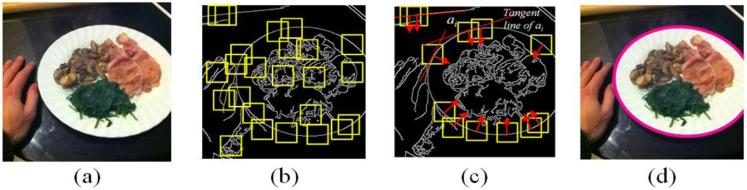
\includegraphics{Figures/2/segm_03.jpg}
\caption{Container detection}
\label{fig:3}
\end{figure}

The main limitation of this approach is that in some cases food is served not in a round shaped container e.g.: take away food box, lunch box which is usually rectangular. Some of the foods can also be eaten without using any container at all e.g: fruits, vegetables.

\iffalse
\section{Food-101 Mining Discriminative components with random forests}
This paper address the problem of automatically recognizing pictured dishes. A novel method is proposed to mine discriminative parts using Random Forests, which allowed to mine for parts simultaneously for all classes and to share knowledge among them.
A dataset of 101 food categories, with 101’000 images, was created by the authors of the paper.  Random forest classification method produced an average accuracy of 50.76 percent.
\fi
\section{Survey of Applications for Counting Calories}

To get a better understanding what are the input methods offered by currently available calorie counter it was decided to try them. To download the apps keyword \"calorie counting\" was entered into the search bar of Google Play Store. The top 3 apps in the search results were downloaded and tested. These apps were MyFitnessPal, Nutracheck, and Lifesum.

MyfitnessPal is the most popular calories Counting app on the Google Play Store. The app has over 50 million downloads on Google Play Store \autoref{fig:mfp}. When the app is launched for the first time the user is required to sign up. After entering his email and password the user has to complete a short survey about his goal, physical activity levels, gender, birthday, location, weight, and height, desired weight and agree to the privacy policy and terms \autoref{fig:mfp2}. After that, the app calculates target daily calorie intake. For entering food user can scan the barcode of the food or use the text-based search. Food search and barcode scanning only work when a phone is connected to the Internet.  The database of food items is quite big and includes products from many different restaurants. However,  adding a meal that was prepared by the user himself is complicated. Every ingredient of a dish must be searched and added separately.  The portion size has to be entered using weight measurements e.g.:  grams. It is often hard to estimate how much does a meal weight so it is a big disadvantage.
 
\begin{figure}[ht]
\centering

\includegraphics[width=5cm,scale=0.5]{Figures/2/mfp1.png}
\caption{Google Play Store page of MyFitnessPal app}
\label{fig:mfp}
\end{figure}

\begin{figure}[ht]
\centering
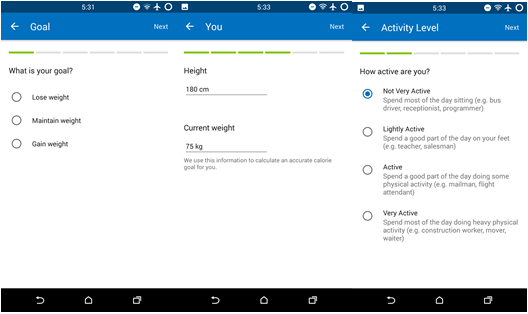
\includegraphics[width=10cm]{Figures/2/mfp2.png}
\caption{Procedure to create a MyFitnessPal account}
\label{fig:mfp2}
\end{figure}

\begin{figure}[ht]
\centering
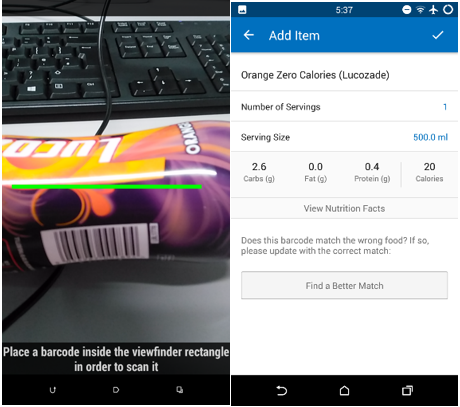
\includegraphics{Figures/2/mfp3.PNG}
\caption{Barcode scanning with MyFitnessPal}
\label{fig:mfp2}
\end{figure}

The other app tested was Nutracheck. To start using Nutracheck a user is required to create an account. The registration procedure is very similar to MyFitnessPal's. For entering meals, the app also has a barcode scanner and search function.  The advantage that Nutracheck has over MyFitnessPal is that it displays images of food in the search results \autoref{fig:eat}. However, a  barcode scanner of this app recognized fewer barcodes that a barcode scanner in MyFitnessPal.

Final app that was tested was Lifesum. It also requires completing a survey in order to start using it and uses a barcode scanner and a search function for adding food. An interesting feature that this app has compared to other apps is food quality rating. It rates a quality of a food according to it nutrition facts and presents the user with a rank of food from A to F \autoref{fig:life}.

 \begin{figure}[ht]
\centering
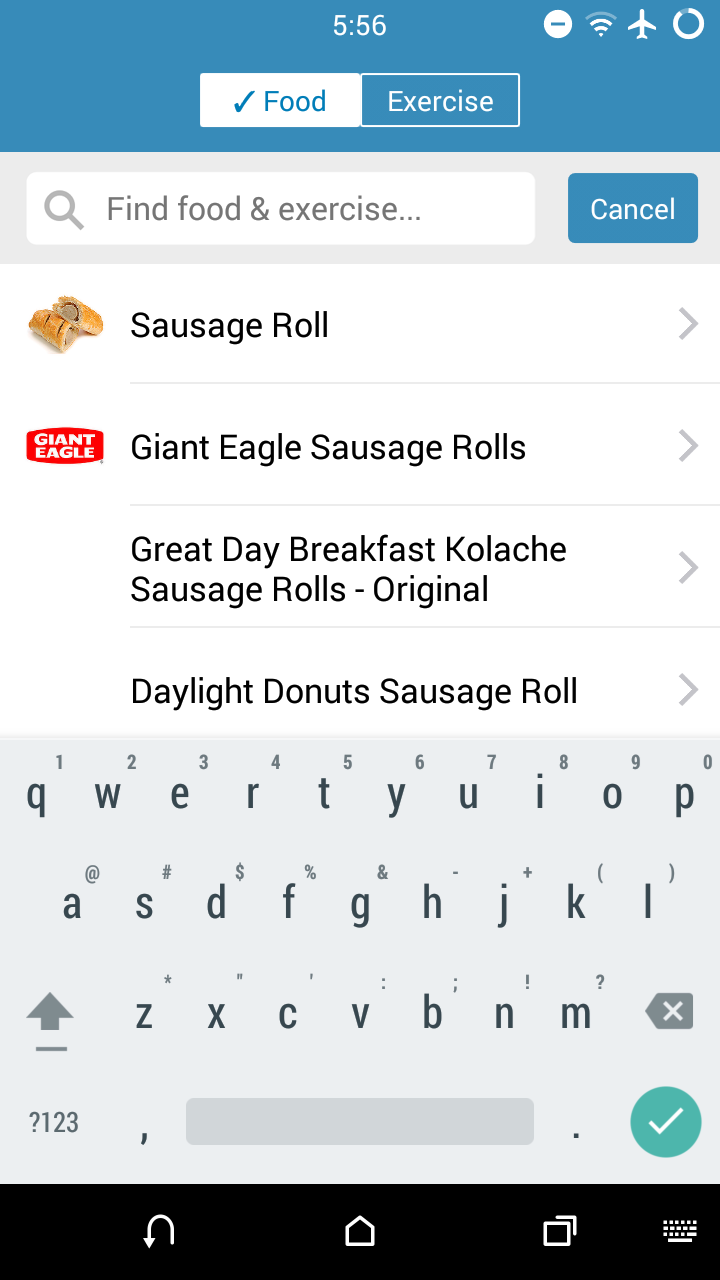
\includegraphics[width=5cm]{Figures/2/eat.png}
\caption{Food database search in Nutracheck}
\label{fig:eat}
\end{figure}

\begin{figure}[ht]
\centering
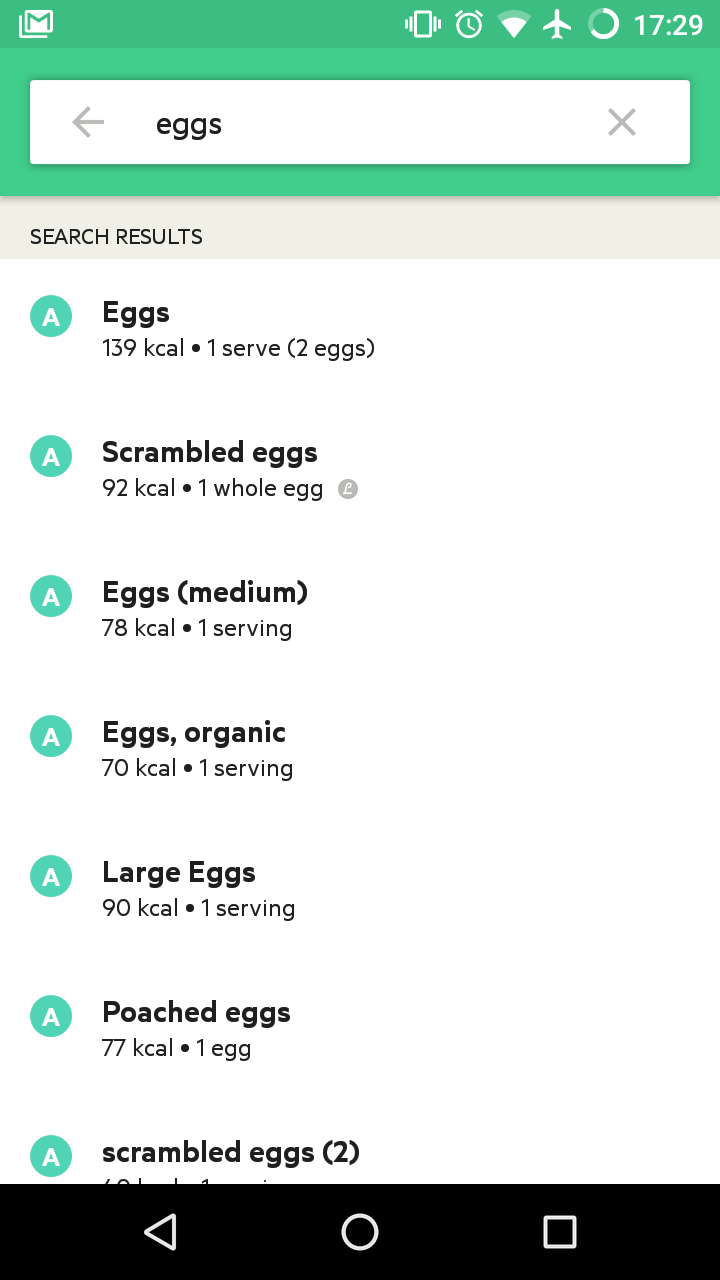
\includegraphics[width=5cm]{Figures/2/mm.png}
\caption{Food database search in LifeSum}
\label{fig:life}
\end{figure}

From this short survey, it can be concluded that currently, available calorie counting apps lack innovation. They all use text-based search and barcode scanners as data entry points. If one wants to track his food, he must remember what did he eat and estimate how much did It weight. All tried apps require an Internet connection for entering food for tracking.  It is clear, that food tracking applications could benefit from a model that can recognize and classify food from images.

\section{Summary}
In this chapter history of computer vision was reviewed. Then, it was explained why computer vision is such a hard problem. Finally, a  paper about automatic food image segmentation was summarized and reviewed. This paper explored dietary assessment only focusing on segmenting a food object from a background. An automatic food image classifier could extend the capabilities of personal dietary assessment with wearable devices. In the next chapter research methods of the project is going to be discussed.